\documentclass{resume} % Use the custom resume.cls style

\usepackage[left=0.75in,top=0.6in,right=0.75in,bottom=0.6in]{geometry} % Document margins
\usepackage{graphicx}
\graphicspath{{images/}}
\name{Suraj Mishra} % Your name
\address{Laxmi niwas,Sadanand nagar ,uttan road ,bhayander (west) Thane-401105} % Your address
\address{+918976330107 \\ rockstarsurajrs@gmail.com} % Your phone number and email

\begin{document}
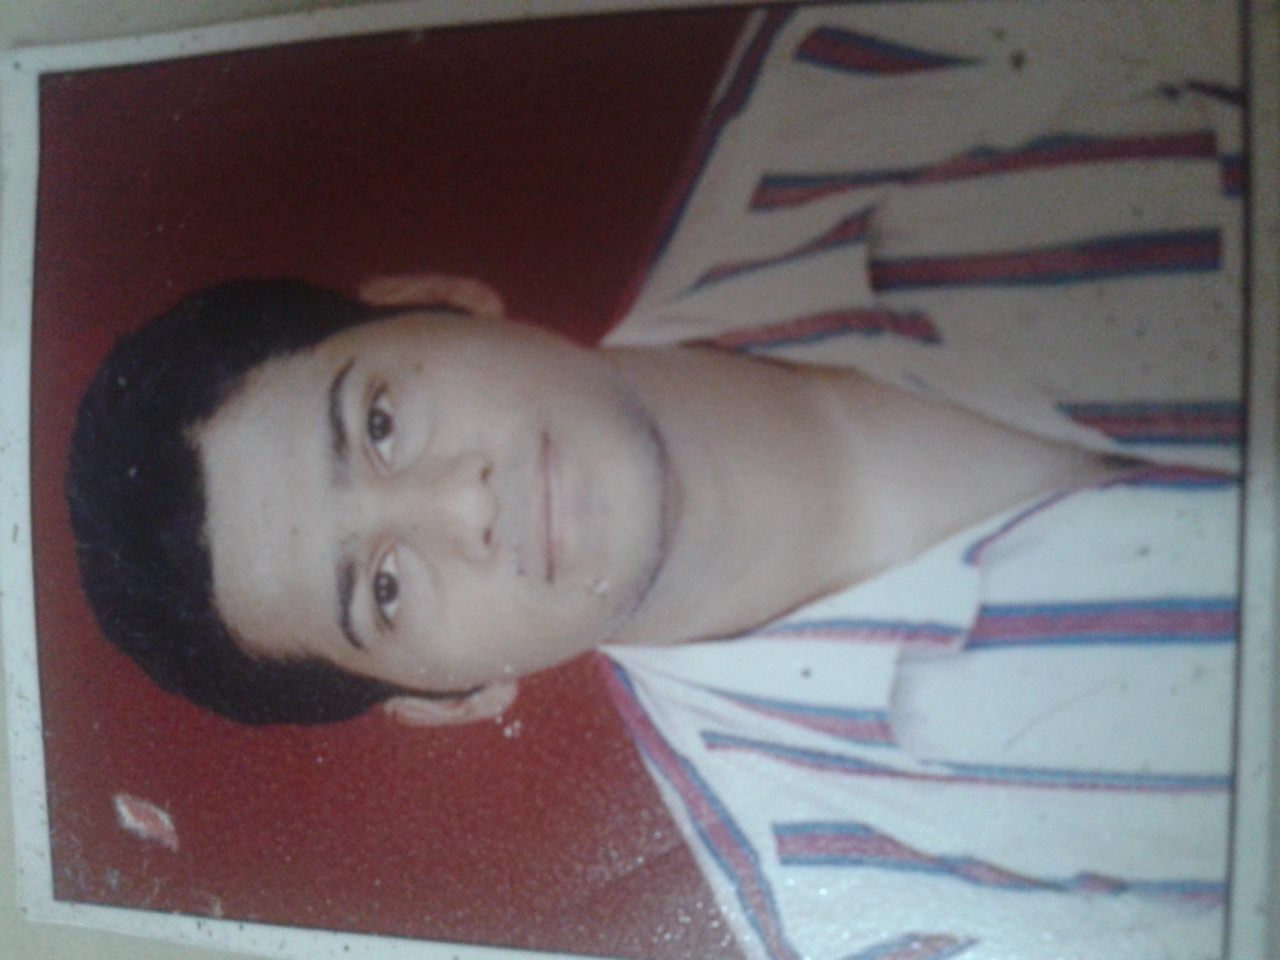
\includegraphics[scale=0.09,angle=270]{4}


\begin{rSection}{Career Objective}
	To seek a challenging  position in the field of IT,where I can exploit my  potential to the fullest and emerge as an effective team member by playing  a proactive role in growth,and grow positive relationship with clients and colleagues at an organization level.
\end{rSection}

\begin{rSection}{Education}
	\begin{center}
		\begin{tabular}{||c|c|c|c||}
			\hline\hline
			\bf Examination & \bf Institute & \bf year & \bf Performance \\
			\hline\hline 
			3rd Year B.Tech & Veermata Jijabai Technological Institute & May, 2015 & 8.2 CGPA \\
			\hline
			H.S.C & K.C college & 2012 & 83.63\% \\
			\hline
			S.S.C & J.H.poddar high school & 2010 & 93.64\% \\
			\hline\hline
			
			
		\end{tabular}
	\end{center}
	
\end{rSection}
\begin{rSection}{Project}
	
	\begin{enumerate}
		\item \begin{rSubsection}{Cargo sorting robot}{embedded}{eyantra,iit bombay}{2015}
			 A robot which detects different cargo's different terminal of airport and place it to proper terminal.
			sensor-color sensor,microcontroller-avr-2560,8.
			Presented in eyantra robotics competition and won first prize among 52  teams.
		\end{rSubsection}
		
		\item \begin{rSubsection}{Blogger Web application} 
			{}{}{} 
		 Successfully made a web application Blogger where user can see authors post,likes or dislikes it and comment on it.Language used were PHP,html and database used was MYsql.   
		\end{rSubsection} 
	\end{enumerate}
\end{rSection}
\begin{rSection}{Training }
	\begin{itemize}
		\item \begin{rSubsection}{CCNA(cisco certified network associate)}{june, 2014}{Networking}{Rst Forum}
			\item 	Trainning of CCNA(cisco certified network associate)  under RST forum, where I learned different
			technology (Ethernet,serial etc) ,communication over such technology,Layer1 devices(like hub ), Layer2 devices(like switch),layer 3 devices(like router).
			\item	Learn concept of subnetting and supernetting and how to use these concept during practical network design.
			\item	Also got exposure to different routing protocols(Like RIP v1\&v2,IGRP,EIGRP,OSPF,ISIS \&BGP),
			Switching protocol(like Spanning tree  protocol(STP),RSTP,VLAN Trunking protocol ).
			
			
		\end{rSubsection}
		
	\end{itemize}
\end{rSection}

\begin{rSection}{Research Publication}
	\begin{enumerate}
		\item Read a research paper on "Vehicle Crash Test using Haar Wavelets" as a part of an academic activity.
		\item No research paper publication yet
	\end{enumerate}
\end{rSection}


\begin{rSection}{Technical Skills}
	\begin{itemize}
		\item programming language-c/c++,PHP;
		\item database-Mysql.
		\item data structure and algorithms
		\item basic of web developement(php,mysql)
		\item embedded programming.
		
	\end{itemize}
\end{rSection}
\begin{rSection}{Soft Skills}
	\begin{enumerate}
		\item good communication skills
		\item good presntation skills
	\end{enumerate}
\end{rSection}
\begin{rSection}{Extra-Curricular Activities}
	\begin{itemize}
		\item \begin{rSubsection}{Contraption}{December, 2014}{Mechanical \& Electroncs}{VJTI, Technovanza}
			\item Event head of Contraption- A mechanical and electronics project and was exhibited at Technovanza Festival
		\end{rSubsection}
		\item \begin{rSubsection}{wall-e }{august, 2013}{Mechanical, Coding \& Electroncis}{sra,vjti}
			\item made sucessfully line following rob ot that tracks black line on white arena.
		\end{rSubsection}
		
	\end{itemize}
\end{rSection}
\begin{rSection}{Co-Curricular activities}
	\begin{enumerate}
		\item Digital Signal Processing on Matlab
		\item Speech Processing on Matlab
		\item Learning Machine Learning Algorithms
	\end{enumerate}
\end{rSection}
\begin{rSection}{Personal Information}
	\item \textbf{Father’s Name:} Sanjay mishra
	\item \textbf{Mother’s Name: } :Lakshmi mishra
	\item \textbf{Sex:} Male
	\item \textbf{Date of Birth:} 15 august,1993 
	\item \textbf{Nationality: } Hindu
	\item \textbf{Marital Status:}	Single
\end{rSection}

\end{document}